\chapter{Experimental Study}\label{ch:4}

\begin{table}[htbp]
\caption{Overview of the experimental stages of Phase I, with the main outcome of each stage after every model was trained to (nearly) 100 \% training accuracy.}\label{tab:4.1}
\small
\begin{tabular}{>{\raggedright\arraybackslash\hspace{0pt}}p{\dimexpr 0.151\linewidth-2\tabcolsep\relax}>{\raggedright\arraybackslash\hspace{0pt}}p{\dimexpr 0.319\linewidth-2\tabcolsep\relax}>{\raggedright\arraybackslash\hspace{0pt}}p{\dimexpr 0.212\linewidth-2\tabcolsep\relax}>{\raggedright\arraybackslash\hspace{0pt}}p{\dimexpr 0.315\linewidth-2\tabcolsep\relax}}
\toprule
\textbf{Stage} & \textbf{Main question} & \textbf{Evaluation} & \textbf{Outcome carried forward} \\
\midrule
Initial project & Can a page-image CNN grade LVEF? & fixed split (168 validation ECGs) & 10 models; CNNs 0.345--0.435, XGBoost 0.494 \\
Phase 1 & Does a foundation ECG model help? & fixed split & ECGFounder fine-tuned 0.560, the best network \\
Phase 2 & Robust re-evaluation, pre-registered & development CV & LGBM-FEAT 0.548; FUSION-MLP macro-F1 0.438 \\
Phase 3 & Fusion and ensembles & development CV & vote ensemble C1 0.517 \\
Phase 4 & EF regression, multitask & development CV & EF $r$ = 0.624; multitask 0.536 \\
Phase 5 & Features, boosting, decision rules & development CV & E2 LightGBM 0.557; C3 selected, 0.533 \\
Phase 6 & Fine-tuning the foundation model & fixed split & ECGFounder fine-tuned 0.560 \\
Label studies & Cleaning and cohorts & CV and subsets & 0.67--0.69 on the clean subsets \\
Phase 7 & Representations and triage & development CV & triage 0.696 on 48 \% of patients \\
Image-only push & HIER, ENH, ULT, EchoNext, SUPER & development CV & ENH-vote 0.549; SUPER-TOP10-ORD 0.558 \\
\bottomrule
\end{tabular}
\end{table}


Phase I was carried out in ten stages (Table~\ref{tab:4.1}). Each stage asked one question, and its lesson was carried into the next. Every model was trained, with the inputs, labels, folds and decision rules of its stage, until its training accuracy reached (nearly) 100 \% (Section~\ref{sec:3.5.3}); the results below are those of 79 classifiers and two EF regressors. Every table is sorted by training accuracy, highest first, and models with the same training accuracy by held-out accuracy. Figure~\ref{fig:6.2} in Chapter~\ref{ch:6} compares all of them.

\section{Initial project and Phase 1}\label{sec:4.1}

\begin{table}[htbp]
\caption{Initial project and Phase 1: image and signal networks on the fixed split (trained on 669 ECGs, validated on 168), every network trained until its training accuracy reached (nearly) 100 \%; sorted by training accuracy, ties by validation accuracy. Best valid. = highest validation accuracy at any epoch on the way to 100 \%. On 168 ECGs the 95 \% interval of an accuracy is about $\pm$0.075.}\label{tab:4.2}
\footnotesize\setlength{\tabcolsep}{3pt}
\begin{tabular}{>{\raggedright\arraybackslash\hspace{0pt}}p{\dimexpr 0.170\linewidth-2\tabcolsep\relax}>{\raggedright\arraybackslash\hspace{0pt}}p{\dimexpr 0.230\linewidth-2\tabcolsep\relax}>{\raggedright\arraybackslash\hspace{0pt}}p{\dimexpr 0.110\linewidth-2\tabcolsep\relax}>{\raggedright\arraybackslash\hspace{0pt}}p{\dimexpr 0.110\linewidth-2\tabcolsep\relax}>{\raggedright\arraybackslash\hspace{0pt}}p{\dimexpr 0.120\linewidth-2\tabcolsep\relax}>{\raggedright\arraybackslash\hspace{0pt}}p{\dimexpr 0.130\linewidth-2\tabcolsep\relax}>{\raggedright\arraybackslash\hspace{0pt}}p{\dimexpr 0.130\linewidth-2\tabcolsep\relax}}
\toprule
\textbf{Model} & \textbf{Layers} & \textbf{Params} & \textbf{Epochs} & \textbf{Training acc.} & \textbf{Validation acc.} & \textbf{Best valid.} \\
\midrule
XGBoost (waveform features) & 2,000 trees on 263 waveform features & -- & -- & 1.000 & 0.494 & -- \\
HOG + RBF-SVM & HOG + PCA-150 + RBF kernel & -- & -- & 1.000 & 0.423 & -- \\
EfficientNet-B0 & 81 conv (16 MBConv) + 1 FC & 4.0 M & 37 & 1.000 & 0.417 & 0.512 \\
1-D SE-ResNet & 37 conv + 1 FC; digitised waveforms & 4.5 M & 32 & 0.999 & 0.435 & 0.542 \\
ECGNet & 29 conv (incl. SE) + 1 FC & 6.3 M & 21 & 0.999 & 0.435 & 0.488 \\
MobileNetV3-Large & 63 conv (15 bottlenecks) + 1 FC & 4.2 M & 57 & 0.999 & 0.387 & 0.476 \\
ResNet-18 & 20 conv + 1 FC (18 weight layers); ImageNet start & 11.2 M & 24 & 0.997 & 0.423 & 0.482 \\
ECGFounder fine-tuned (stages 5--6) & 61 conv + 40 linear (stages 5--6 trained) + 1 FC & 30.7 M & 12 & 0.996 & 0.560 & 0.560 \\
ConvNeXt-Atto & 40 conv (12 blocks) + 1 FC & 3.4 M & 53 & 0.996 & 0.345 & 0.518 \\
Header 0.6 + ResNet-18 0.4 & weighted average (default pipeline of the initial project) & -- & -- & 0.972 & 0.458 & -- \\
Logistic regression (header) & 1 linear layer on the header & -- & -- & 0.674 & 0.405 & -- \\
\bottomrule
\end{tabular}
\end{table}


The initial project compared image and signal models on a fixed split of the development data: classical HOG features with an SVM, CNNs trained from scratch (ECGNet, EfficientNet-B0, MobileNetV3, ConvNeXt-Atto), ImageNet ResNet-18, a 1-D SE-ResNet on digitised waveforms, gradient boosting (XGBoost) on 263 engineered features and the printed header (Table~\ref{tab:4.2}). Trained to (nearly) 100 \%, every network fits its 669 training ECGs (0.996--1.000), but on the 168 validation ECGs the CNNs reach only 0.345--0.435 and the default header + ResNet-18 pipeline 0.458. Every CNN reached its highest validation accuracy (0.476--0.542) before its last epoch. Phase 1 introduced ECGFounder: fine-tuned in stages 5--6, it reaches 0.560 after 12 epochs, the best result on this split, and it became the backbone of later work.

\section{Phases 2--5: robust evaluation, fusion and decision rules}\label{sec:4.2}

\begin{table}[htbp]
\caption{Phases 2--3 and 5: the twelve main models in development cross-validation (5 folds $\times$ 3 repeats, 837 ECGs), each trained to (nearly) 100 \% training accuracy; sorted by training accuracy, ties by held-out accuracy. Held-out accuracy: mean of the 15 test folds with the corrected 95 \% CI; F1, balanced accuracy and recall from the confusion matrix pooled within each repeat. HF AUC = heart-failure screen, reduced EF against Normal (C3 and IMG-C3 use the probabilities of C1 and IMG-vote). $^{\dagger}$ Selective: scored on the patients it answers (share in brackets).}\label{tab:4.3}
\scriptsize\setlength{\tabcolsep}{3pt}
\begin{tabular}{>{\raggedright\arraybackslash\hspace{0pt}}p{\dimexpr 0.150\linewidth-2\tabcolsep\relax}>{\raggedright\arraybackslash\hspace{0pt}}p{\dimexpr 0.100\linewidth-2\tabcolsep\relax}>{\raggedright\arraybackslash\hspace{0pt}}p{\dimexpr 0.200\linewidth-2\tabcolsep\relax}>{\raggedright\arraybackslash\hspace{0pt}}p{\dimexpr 0.080\linewidth-2\tabcolsep\relax}>{\raggedright\arraybackslash\hspace{0pt}}p{\dimexpr 0.075\linewidth-2\tabcolsep\relax}>{\raggedright\arraybackslash\hspace{0pt}}p{\dimexpr 0.075\linewidth-2\tabcolsep\relax}>{\raggedright\arraybackslash\hspace{0pt}}p{\dimexpr 0.075\linewidth-2\tabcolsep\relax}>{\raggedright\arraybackslash\hspace{0pt}}p{\dimexpr 0.245\linewidth-2\tabcolsep\relax}}
\toprule
\textbf{Model} & \textbf{Training acc.} & \textbf{Held-out acc. [95 \% CI]} & \textbf{Macro F1} & \textbf{Mild F1} & \textbf{Bal. acc.} & \textbf{HF AUC} & \textbf{Recall N / Mi / Mo / S} \\
\midrule
Image-only triage$^{\dagger}$ & 1.000 (58 \%) & 0.696 [0.630, 0.762] (48 \%) & 0.372 & 0.049 & 0.367 & -- & 0.99 / 0.03 / 0.19 / 0.27 \\
LGBM-FEAT & 1.000 & 0.548 [0.512, 0.583] & 0.409 & 0.227 & 0.413 & 0.824 & 0.88 / 0.18 / 0.39 / 0.21 \\
FUSION-MLP & 1.000 & 0.538 [0.499, 0.578] & 0.438 & 0.255 & 0.440 & 0.831 & 0.79 / 0.24 / 0.42 / 0.31 \\
ECGF-MLP & 1.000 & 0.536 [0.506, 0.565] & 0.430 & 0.282 & 0.430 & 0.835 & 0.79 / 0.27 / 0.41 / 0.26 \\
IMG-C3 & 1.000 & 0.532 [0.492, 0.572] & 0.416 & 0.252 & 0.413 & 0.822 & 0.82 / 0.23 / 0.38 / 0.22 \\
C1 & 1.000 & 0.517 [0.477, 0.558] & 0.426 & 0.265 & 0.426 & 0.824 & 0.76 / 0.26 / 0.38 / 0.32 \\
IMG-vote & 1.000 & 0.503 [0.463, 0.544] & 0.416 & 0.275 & 0.415 & 0.822 & 0.72 / 0.28 / 0.39 / 0.27 \\
ECGF-linear & 1.000 & 0.491 [0.451, 0.532] & 0.408 & 0.282 & 0.407 & 0.777 & 0.70 / 0.29 / 0.36 / 0.28 \\
C3 & 0.995 & 0.533 [0.496, 0.569] & 0.423 & 0.260 & 0.419 & 0.824 & 0.81 / 0.24 / 0.39 / 0.24 \\
CLIN-LR & 0.720 & 0.442 [0.390, 0.493] & 0.376 & 0.240 & 0.382 & 0.767 & 0.60 / 0.25 / 0.36 / 0.32 \\
HDRCLIN-LR & 0.589 & 0.486 [0.436, 0.536] & 0.415 & 0.252 & 0.429 & 0.786 & 0.68 / 0.24 / 0.35 / 0.45 \\
HDR-LR & 0.529 & 0.483 [0.432, 0.535] & 0.391 & 0.210 & 0.409 & 0.785 & 0.72 / 0.17 / 0.32 / 0.42 \\
\bottomrule
\end{tabular}
\end{table}


\begin{figure}[htbp]
\centering
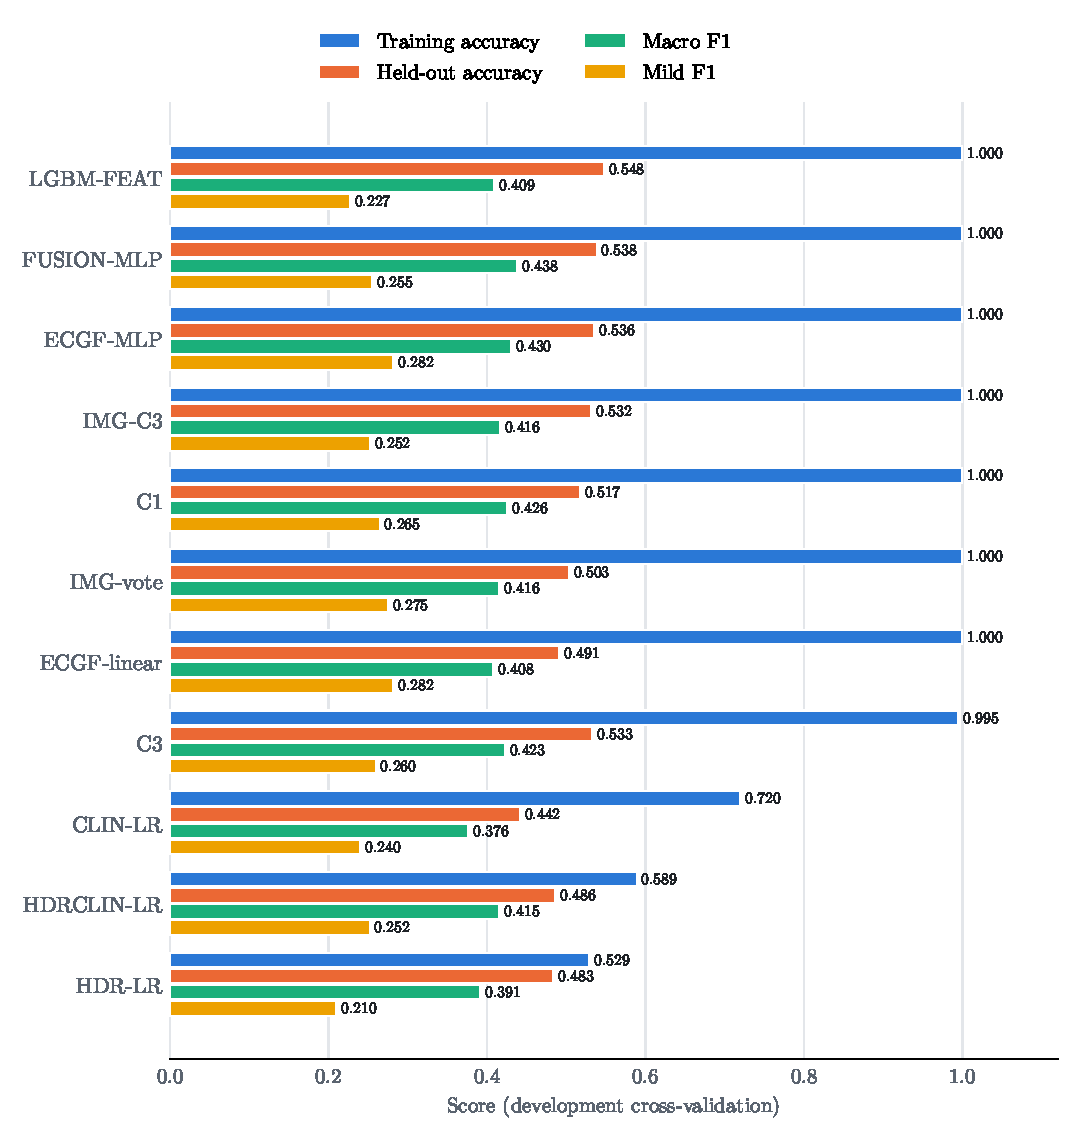
\includegraphics[width=0.90\linewidth,height=0.80\textheight,keepaspectratio]{figures/fig_4_1}
\caption{Training accuracy, held-out accuracy, macro-F1 and Mild F1 of the eleven four-class main models after training to (nearly) 100 \% training accuracy, sorted by training accuracy (development cross-validation).}\label{fig:4.1}
\end{figure}

Phase 2 moved all modelling to pre-registered, patient-grouped cross-validation on the 837 development ECGs (Table~\ref{tab:4.3}, Figure~\ref{fig:4.1}). Nine of the twelve main models reach 1.000 training accuracy and C3 0.995; the three logistic regressions stop at 0.53--0.72 even without regularisation. On held-out patients LightGBM on header and engineered features is the most accurate main model (0.548), FUSION-MLP has the highest macro-F1 (0.438) and balanced accuracy (0.440), and the ECGFounder heads find the Mild class best (Mild F1 0.282). For heart-failure screening (reduced EF against Normal) the ECGFounder-based models reach AUC 0.78--0.84 (ECGF-MLP 0.835) and the header and clinical logistic regressions 0.77--0.79. Phase 3 combined representations: the soft-vote ensemble C1 reaches 0.517.

\begin{table}[htbp]
\caption{Phase 5 experiments in development cross-validation, every model trained to (nearly) 100 \% training accuracy; sorted by training accuracy. Min recall = lowest recall of the four classes (admissible if $\ge$ 0.15). Epochs: median over the 15 folds; $^{b}$ epochs of the member FUSION-MLP.}\label{tab:4.4}
\footnotesize\setlength{\tabcolsep}{3pt}
\begin{tabular}{>{\raggedright\arraybackslash\hspace{0pt}}p{\dimexpr 0.260\linewidth-2\tabcolsep\relax}>{\raggedright\arraybackslash\hspace{0pt}}p{\dimexpr 0.100\linewidth-2\tabcolsep\relax}>{\raggedright\arraybackslash\hspace{0pt}}p{\dimexpr 0.120\linewidth-2\tabcolsep\relax}>{\raggedright\arraybackslash\hspace{0pt}}p{\dimexpr 0.180\linewidth-2\tabcolsep\relax}>{\raggedright\arraybackslash\hspace{0pt}}p{\dimexpr 0.090\linewidth-2\tabcolsep\relax}>{\raggedright\arraybackslash\hspace{0pt}}p{\dimexpr 0.090\linewidth-2\tabcolsep\relax}>{\raggedright\arraybackslash\hspace{0pt}}p{\dimexpr 0.160\linewidth-2\tabcolsep\relax}}
\toprule
\textbf{Experiment} & \textbf{Epochs} & \textbf{Training acc.} & \textbf{Held-out acc. [95 \% CI]} & \textbf{Min recall} & \textbf{Macro F1} & \textbf{Note} \\
\midrule
E2 LightGBM, features + ECGFounder PCA & 2,000 trees & 1.000 & 0.557 [0.517, 0.597] & 0.162 & 0.422 & admissible \\
E1 MLP, header + ECGFounder + feature families & 64 & 1.000 & 0.542 [0.504, 0.579] & 0.238 & 0.442 & admissible \\
E7 mixup MLP & 144 & 1.000 & 0.534 [0.499, 0.570] & 0.243 & 0.434 & admissible \\
E4 hierarchical MLP & 52 / 39 & 0.999 & 0.540 [0.517, 0.563] & 0.223 & 0.433 & admissible \\
E5 vote + nested prior rule (C3) & 112$^{b}$ & 0.995 & 0.533 [0.496, 0.569] & 0.238 & 0.423 & admissible \\
E6 signal-quality gating & 112$^{b}$ & 0.988 & 0.542 [0.500, 0.583] & 0.232 & 0.441 & admissible \\
E3 weighted average of the C1 members & 112$^{b}$ & 0.985 & 0.530 [0.480, 0.581] & 0.223 & 0.428 & admissible \\
E3 stacking (logistic meta-learner) & 112$^{b}$ & 0.826 & 0.532 [0.487, 0.576] & 0.132 & 0.418 & a recall below 0.15 \\
\bottomrule
\end{tabular}
\end{table}


Phase 5 tested engineered features, boosting and decision rules (Table~\ref{tab:4.4}). E2, LightGBM on the engineered features with a 32-component projection of the ECGFounder embedding, is the most accurate (0.557 [0.517, 0.597]). The selected model C3, a vote ensemble with a nested class-prior rule, reaches 0.533 with every class detected.

\section{Phases 4 and 6: EF regression, multitask learning and fine-tuning}\label{sec:4.3}

\begin{table}[htbp]
\caption{Phases 4 and 6: EF regression, multitask learning and fine-tuning, every model trained to (nearly) 100 \% training accuracy (EF regressors: training correlation $\approx$ 1); sorted by the training score. Development cross-validation unless stated.}\label{tab:4.5}
\footnotesize\setlength{\tabcolsep}{3pt}
\begin{tabular}{>{\raggedright\arraybackslash\hspace{0pt}}p{\dimexpr 0.300\linewidth-2\tabcolsep\relax}>{\raggedright\arraybackslash\hspace{0pt}}p{\dimexpr 0.150\linewidth-2\tabcolsep\relax}>{\raggedright\arraybackslash\hspace{0pt}}p{\dimexpr 0.110\linewidth-2\tabcolsep\relax}>{\raggedright\arraybackslash\hspace{0pt}}p{\dimexpr 0.120\linewidth-2\tabcolsep\relax}>{\raggedright\arraybackslash\hspace{0pt}}p{\dimexpr 0.120\linewidth-2\tabcolsep\relax}>{\raggedright\arraybackslash\hspace{0pt}}p{\dimexpr 0.200\linewidth-2\tabcolsep\relax}}
\toprule
\textbf{Model} & \textbf{Measure} & \textbf{Epochs} & \textbf{Training} & \textbf{Held-out} & \textbf{Note} \\
\midrule
Multitask MLP (four classes + EF, header + ECGFounder) & four-class accuracy & 131 & 1.000 & 0.536 & held-out 95 \% CI [0.496, 0.577] \\
EF regression, ridge + LightGBM (triage regressor) & EF (correlation $r$) & 4,000 trees & 1.000 & 0.476 & MAE 0.0 / 13.8 EF points \\
ECGFounder fine-tuned (stages 5--6), fixed split & four-class accuracy & 12 & 0.996 & 0.560 & 168 validation ECGs ($\pm$0.075) \\
EF regression MLP (header + ECGFounder) & EF (correlation $r$) & 3,000 (cap) & 0.993 & 0.624 & MAE 2.7 / 11.0 EF points \\
\bottomrule
\end{tabular}
\end{table}


Phase 4 added EF regression from the image (Table~\ref{tab:4.5}). The MLP regressor reproduces the training EF almost exactly ($r=0.993$, mean error 2.7 points) but reaches $r=0.624$ and a mean error of 11.0 points on held-out patients; the ridge + LightGBM regressor used by the triage model fits its training EF exactly and reaches $r=0.476$. Learning the class and the EF together (multitask) gives 0.536. Phase 6 fine-tuned ECGFounder, which gives the best fixed-split result (0.560, Table~\ref{tab:4.2}).

\section{Label-quality and cohort studies}\label{sec:4.4}

\begin{table}[htbp]
\caption{Label-quality and cohort studies with the C3 recipe trained to (nearly) 100 \% training accuracy (development cross-validation); sorted by training accuracy. Accuracy on the subset named, with the recorded labels. Epochs: median of the member FUSION-MLP.}\label{tab:4.6}
\footnotesize\setlength{\tabcolsep}{3pt}
\begin{tabular}{>{\raggedright\arraybackslash\hspace{0pt}}p{\dimexpr 0.290\linewidth-2\tabcolsep\relax}>{\raggedright\arraybackslash\hspace{0pt}}p{\dimexpr 0.170\linewidth-2\tabcolsep\relax}>{\raggedright\arraybackslash\hspace{0pt}}p{\dimexpr 0.110\linewidth-2\tabcolsep\relax}>{\raggedright\arraybackslash\hspace{0pt}}p{\dimexpr 0.120\linewidth-2\tabcolsep\relax}>{\raggedright\arraybackslash\hspace{0pt}}p{\dimexpr 0.120\linewidth-2\tabcolsep\relax}>{\raggedright\arraybackslash\hspace{0pt}}p{\dimexpr 0.190\linewidth-2\tabcolsep\relax}}
\toprule
\textbf{Study} & \textbf{Scored on} & \textbf{Epochs} & \textbf{Training acc.} & \textbf{Accuracy} & \textbf{Finding} \\
\midrule
NF: noise-free training (all classes) & 264 clean, clear-cut ECGs & 45$^{b}$ & 1.000 & 0.673 & clean labels are graded well \\
HC30: train on exact-name links within 30 days & 395 reliable links & 52$^{b}$ & 1.000 & 0.583 & reliable links give about 0.58 \\
CLEAR: train without the 255 border ECGs & 582 clear-cut ECGs & 104$^{b}$ & 0.993 & 0.670 & clear cases are graded well \\
VER: 15 labels corrected to a high-confidence echo & all 837 & 132$^{b}$ & 0.986 & 0.537 & label noise costs little \\
NFS: noise-free training, Severe kept & 264 clean, clear-cut ECGs & 44$^{b}$ & 0.985 & 0.694 & best on clean labels \\
MMCLEAN: drop 217 suspect Mild or Moderate labels & 620 kept ECGs & 95$^{b}$ & 0.978 & 0.669 & accuracy follows label clarity \\
\bottomrule
\end{tabular}
\end{table}


Pre-registered studies asked whether cleaner labels or reliable cohorts lift performance (Table~\ref{tab:4.6}). On ECGs with clear or verified labels the C3 recipe scores in the upper 60s: 0.670 on 582 clear-cut ECGs, 0.669 on the 620 ECGs kept after removing suspect Mild and Moderate labels, and 0.694 on 264 clean, clear-cut ECGs. Trained on reliable links only it reaches 0.583, and correcting 15 labels gives 0.537 on all ECGs. Clinician-style features identified interpretable Mild markers: a spatial QRS--T angle above 100$^{\circ}$ in 52 \% of Mild against 20 \% of Normal ECGs, and poor R-wave progression in 31 \% against 7 \%.

\section{Phase 7 and the image-only models}\label{sec:4.5}

\begin{table}[htbp]
\caption{Image-only four-class models (no printed header; all 837 ECGs, development cross-validation), every model trained to (nearly) 100 \% training accuracy; sorted by training accuracy. $^{c}$ Epochs of the member ECGF-MLP; solver = fitted to convergence.}\label{tab:4.7}
\footnotesize\setlength{\tabcolsep}{3pt}
\begin{tabular}{>{\raggedright\arraybackslash\hspace{0pt}}p{\dimexpr 0.310\linewidth-2\tabcolsep\relax}>{\raggedright\arraybackslash\hspace{0pt}}p{\dimexpr 0.110\linewidth-2\tabcolsep\relax}>{\raggedright\arraybackslash\hspace{0pt}}p{\dimexpr 0.120\linewidth-2\tabcolsep\relax}>{\raggedright\arraybackslash\hspace{0pt}}p{\dimexpr 0.180\linewidth-2\tabcolsep\relax}>{\raggedright\arraybackslash\hspace{0pt}}p{\dimexpr 0.180\linewidth-2\tabcolsep\relax}>{\raggedright\arraybackslash\hspace{0pt}}p{\dimexpr 0.100\linewidth-2\tabcolsep\relax}}
\toprule
\textbf{Model} & \textbf{Epochs} & \textbf{Training acc.} & \textbf{Held-out acc. [95 \% CI]} & \textbf{Recall N / Mi / Mo / S} & \textbf{Macro F1} \\
\midrule
ENH-vote (6 members, tuned class weights) & 108$^{c}$ & 1.000 & 0.549 [0.513, 0.585] & 0.87 / 0.18 / 0.40 / 0.24 & 0.418 \\
ULT M9 $k$-nearest neighbours ($k$ = 15) & none (kNN) & 1.000 & 0.546 [0.520, 0.571] & 0.90 / 0.13 / 0.43 / 0.11 & 0.382 \\
ULT M10 gradient boosting & 2,000 iter. & 1.000 & 0.540 [0.496, 0.585] & 0.86 / 0.19 / 0.39 / 0.21 & 0.409 \\
HIER two-stage (Normal / middle / Severe, then Mild vs Moderate) & 108$^{c}$ & 1.000 & 0.535 [0.488, 0.582] & 0.82 / 0.18 / 0.42 / 0.30 & 0.426 \\
ENH M5 logistic regression on the HIER inputs & solver & 1.000 & 0.501 [0.450, 0.553] & 0.71 / 0.29 / 0.38 / 0.26 & 0.417 \\
ENH M2 synthetic 10-s ECG $\rightarrow$ ECGFounder & solver & 1.000 & 0.489 [0.439, 0.539] & 0.69 / 0.27 / 0.40 / 0.26 & 0.404 \\
ENH M4 MiniRocket & solver & 1.000 & 0.469 [0.423, 0.515] & 0.67 / 0.22 / 0.36 / 0.34 & 0.390 \\
ENH M3 median-beat shape model & solver & 1.000 & 0.412 [0.358, 0.466] & 0.59 / 0.23 / 0.30 / 0.27 & 0.345 \\
ULT M8 logistic regression, multi-scale ECGFounder & solver & 1.000 & 0.496 [0.459, 0.532] & 0.75 / 0.25 / 0.34 / 0.25 & 0.399 \\
ULT-stack (10 members + predicted EF) & 108$^{c}$ & 0.794 & 0.537 [0.500, 0.574] & 0.87 / 0.21 / 0.31 / 0.25 & 0.409 \\
ULT M12 zone logistic regression & solver & 0.624 & 0.349 [0.302, 0.396] & 0.29 / 0.49 / 0.51 / 0.00 & 0.278 \\
ENH M6 EF ridge $\rightarrow$ EF bands & exact & 0.557 & 0.477 [0.458, 0.496] & 0.91 / 0.00 / 0.00 / 0.56 & 0.257 \\
\bottomrule
\end{tabular}
\end{table}


Phase 7 built header-free cascades. The triage model AGT-img answers only when its EF grade agrees with the image-only classifier IMG-C3 and the EF estimate is far from every class limit: it is correct for \textbf{0.696 of the 48 \%} of ECGs it answers (Table~\ref{tab:4.3}). The image-only models of Table~\ref{tab:4.7} use no printed measurement. Most of them fit their training folds perfectly, and the best, ENH-vote, reaches 0.549 [0.513, 0.585], above the header-using C3 (0.533); the $k$-nearest-neighbour member gives 0.546. Combiners fitted on out-of-fold member outputs (ULT-stack, 0.794) and the EF-band models (0.557--0.624) stay below 1.000 in training.
